%  Assembler.tex
%  Document created by seblovett on hind.ecs.soton.ac.uk
%  Date created: Thu 27 Mar 2014 10:13:13 GMT
%  <+Last Edited: Fri 02 May 2014 11:23:13 BST by hl13g10 on celery +>

\section{Assembler}\label{sect:assembler}
The current instruction set architecture includes an assembler for converting assembly language into hexadecimal. 
This chapter outlines the required formatting and available features of this assembler. 

\subsection{Instruction Formatting}
Each instruction must be formatted using the following syntax. 
Here ``[\dots]'' indicates an optional field:

\begin{center}\texttt{[.LABELNAME] MNEMONIC, OPERANDS, ..., :[COMMENTS]}\end{center}
For example:
\begin{center}\texttt{.loop ADDI, R5, R3, \#5 :Add 5 to R3}
\end{center}

 Comments may be added by preceding them with either : or ;\\

 Accepted general purpose register values are: R0, R1, R2, R3, R4, R5, R6, R7, SP. These can be upper or lower case and SP is equivalently evaluated to R7.\\

 Branch instructions take a symbolic reference to the destination. 
Each type of branch supports moving up to 127 lines forward, or 128 lines backwards. But if a branch is over this limitation, the assembler will automatically create additional instructions to enable greater distances. Each additional branch added will cause two more lines of code to be added to the outputted file. \\

 All label names must begin with a `.' while \texttt{.ISR}/\texttt{.isr} and \texttt{.define} are special cases used for the ISR and variable definitions respectively. \\

 Instruction-less or comments only lines are allowed within the assembly file. \\
\newpage
 {\bf Special Case Label}

 The .ISR/.isr label is reserved for the Interrupt Service Routine and may be located anywhere within the file but must finish with a \textbf{RETI} instruction. There is no restriction on size of the service routine.
Branches may occur within the ISR, but are not allowed into this service routine with the exception of a return from a separate subroutine. For ISR set-up code to be added successfully, there must be at least one unused register within the first 11 lines of the program file, excluding .define statements and the ISR.
%As a result of the positioning of the ISR, any stack initialization must occur within the first 10 lines of main program code since jumping over the ISR requires use of the stack. If not initialized, the default address of the stack pointer is 2047. \\

\subsection{Assembler Directives}
%There is one supported assembler directive  for assigning meaningful names to each of the general purpose registers. 
Symbolic label names are supported for branch-type instructions. Following the previous syntax definition for `.LABELNAME', they can be used instead of numeric branching provided they branch no further than the maximum distance allowed for the instruction used. 
Definitions are supported by the assembler. 
They are used to assign meaningful names to the GPRs to aid with programming.
Definitions can occur at any point within the file and create a mapping from that point onwards. 
Different names can be assigned to the same register, but only one is valid at a time. \\


 The accepted syntax for definitions is:

\begin{center}\texttt{.define NAME REGISTER}\end{center}

\subsection{Running The Assembler}\label{sect:runningassembler}
%The assembler reads a `.asm' file and outputs a `.hex' file in hexadecimal format. 
%It is run by typing ``./assemble filename'' at the command line when in the directory of both the assembler executable and the program assembly file. ``filename'' does not have to include the .asm file extension. 
%The outputted file is saved to the same directory as the input file. \\

The assembler is a python executable and is run by typing ``./assemble.py''. 
Alternatively, the assembler can be placed in a folder on the users path and executed by running ``assemble.py''.
It supports Python versions 2.4.3 to 2.7.3.
A help prompt is given by the script if the usage is not correct, or given a \texttt{-h} or \texttt{--help} argument. 

By default, the script will output the assembled hex to a file with the same name, but with a `.hex' extension in the same directory.
The user can specify a different file to use by using a \texttt{-o filename.hex} or \texttt{--output=filename.hex} argument to the script.
The output file can also be a relative or absolute path to a different directory. 

The full usage for the script is seen in listing~\ref{lst:assemblerusage}. 
This includes the basic rules for writing the assembly language and a version log. 

%\lstinputlisting[label=lst:assemblerusage,caption={Assembler help prompt}]{asmhelp.txt}

%\newpage
\subsection{Error Messages}
This is a list of all the error messages produced by the assembler. 
Each time an error is thrown, the error number, a brief description and the line it occurred on is displayed before exiting. 
A `f' corresponds to a line number in the assembly file, and a `p' corresponds to the pre-processed code list displayed on screen. 
Figure~\ref{fig:AssErrorEx} shows an example screen shot of an error message.


%\begin{figure}
%	\includegraphics{error1screenshot.jpg}
%	\caption{Error1 Example Screen Shot}
%	\label{fig:AssErrorEx}
%\end{figure}
\lstinputlisting[label=lst:assemblerusage,caption={Assembler help prompt}]{asmhelp.txt}
\begin{figure}[h]
	\includegraphics{Figures/error1screenshot.jpg}
	\caption{Error1 Example Screen Shot}
	\label{fig:AssErrorEx}
\end{figure}

\begin{center}
	\centering
	\begin{tabular}{r|p{12cm}}
		\multicolumn{1}{c}{\bf Code} & \multicolumn{1}{c}{\bf Description} \\
		\hline\hline
		ERROR1& Instruction mnemonic is not recognised \\
		ERROR2& Register code within instruction is not recognised\\
		ERROR3& Branch condition code is not recognised\\
		ERROR4& Attempting to branch to undefined location \\
		ERROR5& Instruction mnemonic is not recognised \\
		ERROR6& Attempting to shift by more than 16 or perform a negative shift \\
		ERROR7& Magnitude of immediate value for ADDI, ADCI, SUBI, SUCI, LDW, STW, CMPI or JMP is too large\\
		ERROR8& Magnitude of immediate value for ADDIB, SUBIB, LUI or LLI is too large \\
		ERROR9& Attempting to jump more than 127 forward or 128 backwards \\
		ERROR10& Duplicate symbolic link names \\
		ERROR11& Illegal branch to ISR \\
		ERROR12& Multiple ISRs in file \\
		ERROR13& Invalid formatting for .define directive \\
		ERROR14& Could not find empty register in first 10 lines for automated ISR setup \\
		ERROR15& Instruction does not have enough operands \\
	\end{tabular}
\end{center}
